% ============================================================
%  SCHOLA DOMESTICA — Magister Mathematica
%  Level 1 | Week 12 | Day 2
%  Topic: Subtraction Facts — −2 and −3 from 6 and Under
% ============================================================
\documentclass[12pt, letterpaper]{article}

\usepackage[top=1in, bottom=1in, left=1in, right=1in]{geometry}
\usepackage[T1]{fontenc}
\usepackage[utf8]{inputenc}
\usepackage{lmodern}
\usepackage{microtype}
\usepackage{amsmath}
\usepackage{xcolor}
\usepackage{tikz}
\usepackage{array}
\usepackage{enumitem}
\usepackage{multicol}
\usepackage{mdframed}
\usepackage{fancyhdr}

\definecolor{scholared}{RGB}{160,30,30}
\definecolor{scholagold}{RGB}{180,140,40}
\definecolor{scholacream}{RGB}{253,248,235}
\definecolor{scholagreen}{RGB}{50,110,60}
\definecolor{scholablue}{RGB}{40,80,140}

\pagestyle{fancy}
\fancyhf{}
\renewcommand{\headrulewidth}{0.6pt}
\fancyhead[L]{\small\textcolor{scholared}{\textbf{Schola Domestica — Magister Mathematica}}}
\fancyhead[R]{\small\textcolor{scholared}{Level 1 · Week 12 · Day 2}}
\fancyfoot[C]{\small\textcolor{gray}{— \thepage\ —}}

\newcommand{\answerline}{\underline{\hspace{2.5cm}}}
\newcommand{\biganswerline}{\underline{\hspace{4cm}}}
\newcommand{\numbox}{\tikz{\draw[scholablue,thick](0,0)rectangle(1.2cm,0.85cm);}}

\newmdenv[
  backgroundcolor=scholacream,
  linecolor=scholared,
  linewidth=1.5pt,
  roundcorner=6pt,
  innertopmargin=8pt,
  innerbottommargin=8pt,
  innerleftmargin=10pt,
  innerrightmargin=10pt
]{lessonbox}

\newmdenv[
  backgroundcolor={rgb,255:red,235;green,245;blue,235},
  linecolor=scholagreen,
  linewidth=1.2pt,
  roundcorner=4pt,
  innertopmargin=6pt,
  innerbottommargin=6pt,
  innerleftmargin=8pt,
  innerrightmargin=8pt
]{enrichbox}

\begin{document}

\begin{center}
  {\LARGE\textbf{\textcolor{scholared}{Subtraction Facts:}}}\\[4pt]
  {\Large\textcolor{scholagold}{\textit{Taking Away Two and Three}}}\\[6pt]
  {\small Name: \biganswerline \hspace{1cm} Date: \answerline}
\end{center}

\vspace{4pt}
\noindent\textcolor{scholared}{\rule{\linewidth}{1pt}}
\vspace{4pt}

% IMAGE PROMPT (Beatrix Potter watercolour style):
% A mouse reaches into a pouch of seeds and removes three, placing them on a leaf beside the pouch.
% The remaining seeds are visible inside. Warm golden tones, white paper background, no text.

\begin{lessonbox}
\textbf{Counting back} is the strategy for $-2$ and $-3$:\\[4pt]
\begin{itemize}[leftmargin=1.5em, itemsep=3pt]
  \item $5 - 2$: start at 5, count back 2 → \textit{four} … \textit{three} $= 3$
  \item $6 - 3$: start at 6, count back 3 → \textit{five} … \textit{four} … \textit{three} $= 3$
\end{itemize}
\medskip
\noindent\textbf{Tip:} Use your fingers to track each step back.
\end{lessonbox}

\bigskip

% ===== PART I: −2 ON NUMBER LINE =====
\noindent\textcolor{scholared}{\large\textbf{Part I — Subtracting Two}} \hfill \textit{(Problems 1–5)}

\medskip
\noindent\textit{Hop 2 spaces to the \textbf{left} on the number line. Write the difference.}

\bigskip

\noindent
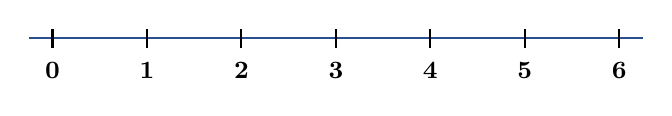
\begin{tikzpicture}
  \draw[thick, scholablue] (0,0) -- (7.8,0);
  \foreach \n in {0,...,6} {
    \draw[thick] (\n*1.2+0.3,-0.12)--(\n*1.2+0.3,0.12);
    \node[below] at (\n*1.2+0.3,-0.18) {\small\textbf{\n}};
  }
\end{tikzpicture}

\bigskip

\noindent
\begin{tabular}{@{}p{3.5cm} p{3.5cm} p{3.5cm} p{3.5cm}@{}}
\textbf{1.}\; $2 - 2 =$ \numbox &
\textbf{2.}\; $3 - 2 =$ \numbox &
\textbf{3.}\; $4 - 2 =$ \numbox &
\textbf{4.}\; $5 - 2 =$ \numbox
\end{tabular}

\medskip
\noindent\textbf{5.}\; $6 - 2 =$ \numbox

\bigskip\bigskip

% ===== PART II: −3 WITH CROSS-OUT =====
\noindent\textcolor{scholared}{\large\textbf{Part II — Subtracting Three}} \hfill \textit{(Problems 6–10)}

\medskip
\noindent\textit{Cross out 3 dots. Count remaining. Write the difference.}

\bigskip

\noindent
\begin{tabular}{@{}p{7.2cm} p{7.2cm}@{}}
% 6: 3−3=0
\textbf{6.}\quad

\begin{tikzpicture}[baseline=-0.5ex]
  \foreach \i in {1,...,3} {
    \filldraw[scholared!40](\i*0.42,0)circle(0.14cm);
    \draw[scholared,thick]({\i*0.42-0.13},-0.13)--({\i*0.42+0.13},0.13);
    \draw[scholared,thick]({\i*0.42-0.13},0.13)--({\i*0.42+0.13},-0.13);
  }
\end{tikzpicture}
\quad $3 - 3 =$ \numbox
&
% 7: 4−3=1
\textbf{7.}\quad

\begin{tikzpicture}[baseline=-0.5ex]
  \filldraw[scholablue](0.42,0)circle(0.14cm);
  \foreach \i in {2,3,4} {
    \filldraw[scholared!40](\i*0.42,0)circle(0.14cm);
    \draw[scholared,thick]({\i*0.42-0.13},-0.13)--({\i*0.42+0.13},0.13);
    \draw[scholared,thick]({\i*0.42-0.13},0.13)--({\i*0.42+0.13},-0.13);
  }
\end{tikzpicture}
\quad $4 - 3 =$ \numbox \\[18pt]

% 8: 5−3=2
\textbf{8.}\quad

\begin{tikzpicture}[baseline=-0.5ex]
  \foreach \i in {1,2} { \filldraw[scholablue](\i*0.42,0)circle(0.14cm); }
  \foreach \i in {3,4,5} {
    \filldraw[scholared!40](\i*0.42,0)circle(0.14cm);
    \draw[scholared,thick]({\i*0.42-0.13},-0.13)--({\i*0.42+0.13},0.13);
    \draw[scholared,thick]({\i*0.42-0.13},0.13)--({\i*0.42+0.13},-0.13);
  }
\end{tikzpicture}
\quad $5 - 3 =$ \numbox
&
% 9: 6−3=3
\textbf{9.}\quad

\begin{tikzpicture}[baseline=-0.5ex]
  \foreach \i in {1,2,3} { \filldraw[scholablue](\i*0.42,0)circle(0.14cm); }
  \foreach \i in {4,5,6} {
    \filldraw[scholared!40](\i*0.42,0)circle(0.14cm);
    \draw[scholared,thick]({\i*0.42-0.13},-0.13)--({\i*0.42+0.13},0.13);
    \draw[scholared,thick]({\i*0.42-0.13},0.13)--({\i*0.42+0.13},-0.13);
  }
\end{tikzpicture}
\quad $6 - 3 =$ \numbox \\[18pt]

\multicolumn{2}{@{}l@{}}{\textbf{10.}\quad $0 - 0 =$ \numbox \quad \textit{(nothing to take away)}}
\end{tabular}

\bigskip\bigskip

% ===== PART III: MIXED −0, −1, −2, −3 =====
\noindent\textcolor{scholared}{\large\textbf{Part III — Mixed Subtraction from 6}} \hfill \textit{(Problems 11–16)}

\bigskip

\noindent
\begin{tabular}{@{}p{3.3cm} p{3.3cm} p{3.3cm} p{3.3cm}@{}}
\textbf{11.}\; $6 - 2 =$ \numbox &
\textbf{12.}\; $5 - 3 =$ \numbox &
\textbf{13.}\; $4 - 1 =$ \numbox &
\textbf{14.}\; $6 - 0 =$ \numbox \\[12pt]
\multicolumn{2}{@{}l@{}}{\textbf{15.}\; $3 - 2 =$ \numbox} &
\multicolumn{2}{@{}l@{}}{\textbf{16.}\; $6 - 3 =$ \numbox}
\end{tabular}

\bigskip

\begin{enrichbox}
\textbf{\textcolor{scholagreen}{Turn-around partners of subtraction}}\\[3pt]
Every subtraction has a related addition fact:\\[3pt]
$6 - 3 = 3$ \quad because \quad $3 + 3 = 6$ \\
$5 - 2 = 3$ \quad because \quad $3 + 2 = 5$ \\[3pt]
\textit{Knowing addition facts helps you check subtraction!}
\end{enrichbox}

\vspace{0.3cm}
\noindent\textcolor{gray}{\small\textit{Ray's Primary Arithmetic — counting back and using related facts.}}

\end{document}
